\documentclass[12pt]{article}
\usepackage[danish]{babel}
\usepackage{amsfonts, amssymb, mathtools, amsthm, amsmath}
\usepackage{graphicx, pgfplots}
\usepackage{url}
\usepackage[dvipsnames]{xcolor}
\usepackage{sagetex}
\usepackage{lastpage}
\usepackage{wrapfig} 
\usepackage[stretch=10]{microtype}


%loaded last
\usepackage[hidelinks]{hyperref}

\usepackage{siunitx}
  \sisetup{exponent-product = \cdot,
    output-decimal-marker = {,}}

%Giles Castelles incfig
\usepackage{import}
\usepackage{xifthen}
\usepackage{pdfpages}
\usepackage{transparent}

\newcommand{\incfig}[2][1]{%
  \def\svgwidth{#1\columnwidth}
  \import{./figures/}{#2.pdf_tex}
}

\setlength{\parindent}{0in}
\setlength{\oddsidemargin}{0in}
\setlength{\textwidth}{6.5in}
\setlength{\textheight}{8.8in}
\setlength{\topmargin}{0in}
\setlength{\headheight}{18pt}

\usepackage{fancyhdr}
\pagestyle{fancy}

\fancyhead{}
\fancyfoot{}
\fancyfoot[R]{Side \thepage{} af \pageref{LastPage}}
\fancyhead[L]{\footnotesize{Noah Rahbek Bigum Hansen}}

% Redefine the plain page style to be consistent
\fancypagestyle{plain}{
  \fancyhead{} % Clears all header content
  \fancyfoot{} % Clears all footer content
  \renewcommand{\headrulewidth}{0pt} % Removes the horizontal line
  \fancyfoot[R]{Side \thepage{} af \pageref{LastPage}} % Page number in the footer
}

\pgfplotsset{compat=newest}

\pgfplotsset{every axis/.append style={
  axis x line=middle,    % put the x axis in the middle
  axis y line=middle,    % put the y axis in the middle
  axis line style={<->,color=black}, % arrows on the axis
}}

\usepackage{thmtools}
\usepackage{tcolorbox}
  \tcbuselibrary{skins, breakable}
  \tcbset{
    space to upper=1em,
    space to lower=1em,
  }

\theoremstyle{definition}

\newtcolorbox[auto counter]{definition}[1][]{%
  breakable,
  colframe=ForestGreen,  %frame color
  colback=ForestGreen!5, %background color
  colbacktitle=ForestGreen!25, %background color for title
  coltitle=ForestGreen!70!black,  %title color
  fonttitle=\bfseries\sffamily, %title font
  left=1em,              %space on left side in box,
  enhanced,              %more options
  frame hidden,          %hide frame
  borderline west={2pt}{0pt}{ForestGreen},  %display left line
  title=Definition \thetcbcounter: #1,
}

\newtcolorbox{greenline}{%
  breakable,
  colframe=ForestGreen,  %frame color
  colback=white,          %remove background color
  left=1em,              %space on left side in box
  enhanced,              %more options
  frame hidden,          %hide frame
  borderline west={2pt}{0pt}{ForestGreen},  %display left line
}

\newtcolorbox[auto counter, number within=section]{eks}[1][]{%
  brekable,
  colframe=NavyBlue,  %frame color
  colback=NavyBlue!5, %background color
  colbacktitle=NavyBlue!25,    %background color for title
  coltitle=NavyBlue!70!black,  %title color
  fonttitle=\bfseries\sffamily, %title font
  left=1em,            %space on left side in box,
  enhanced,            %more options
  frame hidden,        %hide frame
  borderline west={2pt}{0pt}{NavyBlue},  %display left line
  title=Eksempel \thetcbcounter: #1
}

\newtcolorbox{blueline}{%
  breakable,
  colframe=NavyBlue,     %frame color
  colback=white,         %remove background
  left=1em,              %space on left side in box,
  enhanced,              %more options
  frame hidden,          %hide frame
  borderline west={2pt}{0pt}{NavyBlue},  %display left line
}

\newtcolorbox{teo}[1][]{%
  breakable,
  colframe=RawSienna,  %frame color
  colback=RawSienna!5, %background color
  colbacktitle=RawSienna!25,    %background color for title
  coltitle=RawSienna!70!black,  %title color
  fonttitle=\bfseries\sffamily, %title font
  left=1em,              %space on left side in box,
  enhanced,              %more options
  frame hidden,          %hide frame
  borderline west={2pt}{0pt}{RawSienna},  %display left line
  title=Teori: #1,
}

\newtcolorbox[auto counter, number within=section]{sæt}[1][]{%
  breakable,
  colframe=RawSienna,  %frame color
  colback=RawSienna!5, %background color
  colbacktitle=RawSienna!25,    %background color for title
  coltitle=RawSienna!70!black,  %title color
  fonttitle=\bfseries\sffamily, %title font
  left=1em,              %space on left side in box,
  enhanced,              %more options
  frame hidden,          %hide frame
  borderline west={2pt}{0pt}{RawSienna},  %display left line
  title=Sætning \thetcbcounter: #1,
  before lower={\textbf{Bevis:}\par\vspace{0.5em}},
  colbacklower=RawSienna!25,
}

\newtcolorbox{redline}{%
  breakable,
  colframe=RawSienna,  %frame color
  colback=white,       %Remove background color
  left=1em,            %space on left side in box,
  enhanced,            %more options
  frame hidden,        %hide frame
  borderline west={2pt}{0pt}{RawSienna},  %display left line
}

\newtcolorbox{for}[1][]{%
  breakable,
  colframe=NavyBlue,  %frame color
  colback=NavyBlue!5, %background color
  colbacktitle=NavyBlue!25,    %background color for title
  coltitle=NavyBlue!70!black,  %title color
  fonttitle=\bfseries\sffamily, %title font
  left=1em,              %space on left side in box,
  enhanced,              %more options
  frame hidden,          %hide frame
  borderline west={2pt}{0pt}{NavyBlue},  %display left line
  title=Forklaring #1,
}

\newtcolorbox{bem}{%
  breakable,
  colframe=NavyBlue,  %frame color
  colback=NavyBlue!5, %background color
  colbacktitle=NavyBlue!25,    %background color for title
  coltitle=NavyBlue!70!black,  %title color
  fonttitle=\bfseries\sffamily, %title font
  left=1em,              %space on left side in box,
  enhanced,              %more options
  frame hidden,          %hide frame
  borderline west={2pt}{0pt}{NavyBlue},  %display left line
  title=Bemærkning:,
}

\makeatother
\def\@lecture{}%
\newcommand{\lecture}[3]{
  \ifthenelse{\isempty{#3}}{%
    \def\@lecture{Lecture #1}%
  }{%
    \def\@lecture{Lecture #1: #3}%
  }%
  \subsection*{\makebox[\textwidth][l]{\@lecture \hfill \normalfont\small\textsf{#2}}}
}

\makeatletter

\newcommand{\opgave}[1]{%
 \def\@opgave{#1}%
 \subsection*{Opgave #1}
}

\makeatother

%Format lim the same way in intext and in display
\let\svlim\lim\def\lim{\svlim\limits}

% horizontal rule
\newcommand\hr{
\noindent\rule[0.5ex]{\linewidth}{0.5pt}
}


\title{Afleveringsopgave 7}
\author{Noah Rahbek Bigum Hansen}
\date{5. December 2024}

\begin{document}

\maketitle

\section*{Problem 1/3}
\begin{figure} [ht]
  \centering
  \caption{}
  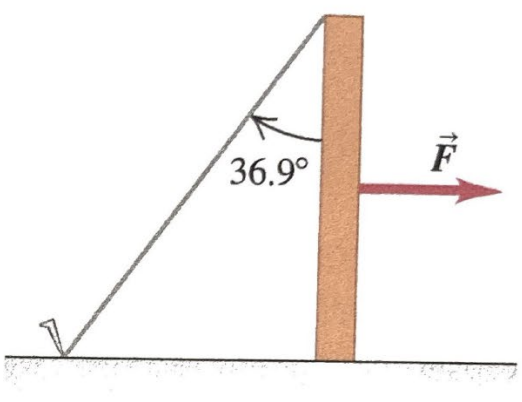
\includegraphics[width=0.5\linewidth]{../figures/P11_90.png}
  \label{fig:P11_90}
\end{figure}
\textbf{Knocking Over a Post.} One end of a post weighing \qty{400}{N} and with height $h$ rests on a rough horizontal surface with $\mu_s = \num{0,30}$. The upper end is held by a rope fastened to the surface and making an angle of \ang{36,9} with the post (\textbf{\autoref{fig:P11_90}}). A horizontal force $\Vec{F}$ is exerted on the post as shown.

\subsection*{(a)}
If the force $\Vec{F}$ is applied at the midpoint of the post, what is the largest value it can have without causing the post to slip?
\begin{figure}[ht]
  \centering
  \incfig[0.8]{A7P1}
  \caption{Fritlegemediagram}
  \label{fig:A7P1}
\end{figure}
\bigbreak
Fra opgaven har vi at $F_t = \qty{400}{N}$, $\mu_s = \num{0,30}$ og $\theta = \ang{36,9}$. Desuden har vi at $f_s = \mu_s N = \num{0,30}N$. Det antages at stangen ikke har nogen tykkelse. 

Idet der er statik indtil kraften bliver for stor har vi ligeledes at summen af kræfterne i alle retninger og alle momenter skal være 0. Vi kan opstille et udtryk for summen af momenterne omkring punkt A (se \textbf{\autoref{fig:A7P1}}) som
\begin{equation} \label{eq:kraft}
  \sum \tau_A = 0 = \frac{h}{2}F - hf_s \implies F = 2f_s = 2 \mu_s N
\end{equation}

Det samme kan nu gøres for momenterne omkring $B$ som
\begin{equation} \label{eq:snorkraft}
\sum \tau_B = 0 = h T_x - \frac{h}{2}F \implies T = \frac{F}{2 \sin\theta}
\end{equation}

Og slutteligt kan det samme gøres for kræfterne i $y$-retningen som
\begin{equation} \label{eq:normalkraft}
  \sum F_y = 0 = N - F_t - T_y \implies N = F_t + \cos (\theta) T
\end{equation} 

Ved indsættelse af \autoref{eq:normalkraft} i \autoref{eq:kraft} fås
\begin{equation} \label{eq:kraft2}
  F = 2 \mu_s \left( F_t + \cos(\theta) T \right)
\end{equation}

Slutteligt kan \autoref{eq:snorkraft} indsættes i \autoref{eq:kraft2} for at få
\[ 
  F = 2 \mu_s \left( F_t + \cos \theta \cdot \frac{F}{2 \sin \theta} \right)
.\]
Kraften $F$ kan nu isoleres som
\begin{gather*}
  F = 2\mu_s F_t + \mu_s \cos \theta \cdot \frac{F}{\sin\theta} \\
  F - \mu_s \cos \theta \cdot \frac{F}{\sin \theta} = 2\mu_s F_t \\
  F \left( 1 - \mu_s \frac{1}{\tan\theta} \right) = 2\mu_s F_t \\
  F = \frac{2\mu_s F_t}{1 - \frac{\mu_s}{\tan \theta}}
.\end{gather*}
Indsættes de kendte størrelser heri kan kraften $F$ der netop ikke får stangen til at bevæge sig findes
\[ 
F = \frac{2 \cdot \num{0,30} \cdot \qty{400}{N}}{1 - \frac{\num{0,3}}{\tan \ang{36,9}}} = \qty{399,709}{N} 
.\]
Altså er den største størrelse som kraften $\Vec{F}$ kan antage uden at pælen begynder at glide \underline{\underline{$F = \qty{0,40}{kN}$}}.


\subsection*{(b)}
How large can the force be without causing the post to slip if its point of application is $\frac{6}{10}$ of the way from the ground to the top of the post?
\bigbreak
Der kan opskrives generelle udtryk for afstanden fra hhv. $A$ og $B$ til kraftens angrebspunkt som
\[ 
l_{FA} = (1-k)h, \qquad l_{FB} = kh
.\]
Hvor værdien af $k$ angiver, hvor på stangen som kraften virker (i denne opgave er $k = \frac{6}{10}$. På samme måde som i (a) kan dermed opstilles tre ligninger som
\begin{align*}
  \sum \tau_A = 0 &= (1-k)h\cdot F - f_s\cdot h \implies F = \frac{\mu_s \cdot N}{1-k} \\
  \sum \tau_B = 0 &= hT_x - kh\cdot F \implies T = \frac{kF}{\sin\theta} \\
  \sum F_y = 0 &= N - F_g - T_y \implies N = F_g + \cos(\theta)T
.\end{align*}
På samme måde som i (a) kan udtrykkene for $\sum F_y$ og $\sum \tau_B$ indsættes i udtrykket for $\sum \tau_A$ som
\[ 
F = \frac{\mu_s \cdot (F_g + \cos(\theta) \cdot \frac{kF}{\sin\theta})}{1-k} = \left( \frac{1}{1-k} \right) \cdot \left( F_g + \cos (\theta) \cdot \frac{kF}{\sin \theta} \right) \mu_s
.\]
På samme måde som i (a) kan kraften nu isoleres
\begin{gather*}
  F = \frac{1}{1-k} \cdot F_g \cdot \mu_s + \frac{1}{1-k} \cdot \cos (\theta) \cdot \frac{kF}{\sin \theta} \mu_s \\
  F - \frac{1}{1-k} \cdot \cos(\theta) \frac{kF}{\sin \theta} \mu_s = \frac{1}{1-k}\cdot F_g\cdot \mu_s \\
  F \left( 1 - \frac{1}{1-k} \cdot \frac{k\mu_s}{\tan \theta} \right) = \frac{1}{1-k} \cdot F_g \cdot \mu_s \\
  F = \frac{\frac{1}{1-k} \cdot F_g \cdot \mu_s}{1 - \frac{1}{1-k}\cdot \frac{k\mu_s}{\tan\theta}} \\
  F = \frac{\frac{1}{1 - \frac{6}{10}} \cdot \qty{400}{N} \cdot \num{0,30}}{1 - \frac{1}{1 - \frac{6}{10}} \cdot \frac{\num{0,30} \cdot \frac{6}{10}}{\tan \ang{36,9}}} = \qty{0,75}{kN} 
.\end{gather*}
Altså er den største størrelse som kraften $\Vec{F}$ kan antage uden at pælen begynder at glide, hvis kraften påføres $\frac{6}{10}$ oppe ad stangens højde \underline{\underline{$F = \qty{0,75}{kN}$}}


\subsection*{(c)}
Show that if the point of application of the force is too high, the post cannot be made to slip, no matter how great the force. Find the critical height for the point of application.
\bigbreak
Fra (b) har vi at kraften der kræves for netop at rykke på stangen er
\[ 
F = \frac{\frac{1}{1-k} \cdot F_g \cdot \mu_s}{1 - \frac{1}{1-k}\cdot \frac{k\mu_s}{\tan\theta}}
.\]
Dette kan vha. alm. brøkregneregler omskrives til
\begin{align*}
  F &= \frac{F_g \cdot \mu_s}{\left( 1-k \right) \cdot \left( 1 - \frac{k\mu_s}{\tan(\theta) (1-k)} \right)} \\
  &= \frac{F_g \cdot \mu_s}{1-k - \frac{k\mu_s}{\tan\theta}}
.\end{align*} 
Kraften går mod uendeligt når nævneren går mod 0, desuden bliver kraften negativ for en nævner mindre end 0 og derfor skal altså findes den værdi af $k$ der medfører at nævneren bliver mindre end eller lig med 0.
\[ 
0 \geq 1-k - \frac{k\mu_s}{\tan\theta}
.\]
Heri kan $k$ isoleres som
\begin{align*}
  0 &\geq 1 - \left( 1 + \frac{\mu_s}{\tan\theta} \right)k \\
  \left( 1 - \frac{\mu_s}{\tan\theta} \right) k &\geq 1 \\
  k &\geq \frac{1}{1 + \frac{\mu_s}{\tan\theta}} \\
  k &\geq \frac{1}{1 + \frac{\num{0,30}}{\tan \ang{36,9}}} = \num{0,71} 
.\end{align*}
Altså kan stangen ikke rykkes, selv med en uendelig stor påført kraft såfremt denne kraft har et angrebspunkt højere end \underline{\underline{\num{0,71} $h$}}. Dette skyldes at snorkraften kommer til at antage en størrelse således at snorkraftens $x$-komposant netop sørger for statik i $x$-retningen. For at den kan dette bliver $y$-komposanten fra snorkraften også større for en større påført kraft $F$. Når kraften $F$ er placeret for højt oppe (højere end \num{0,71}$h$) medvirker snorkraftens $y$-komposant at friktionskraften altid kommer til at kunne ``modstå'' en større kraft end den påførte.



\section*{Problem 2/3}
\begin{figure} [ht]
  \centering
  \caption{}
  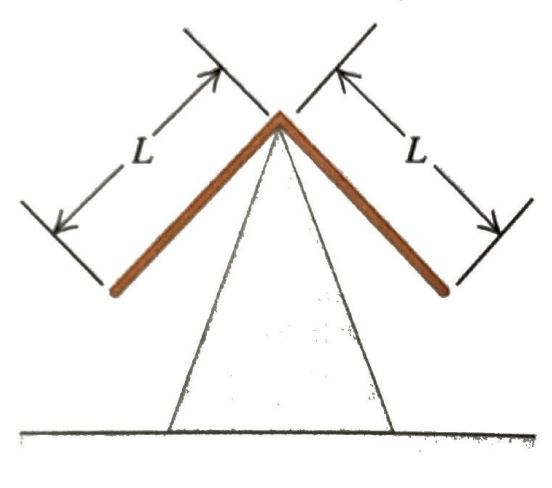
\includegraphics[width=0.5\linewidth]{../figures/P14_88.png}
  \label{fig:P14_88}
\end{figure}
Two identical thin rods each with mass $m$ and length $L$, are joined at right angles to form an L-shaped object. This object is balanced on top of a sharp edge (\textbf{\autoref{fig:P14_88}}). If the L-shaped object is deflected slightly, it oscillates. Find the frequency of oscillation.

\begin{figure}[ht]
  \centering
  \incfig[0.6]{A7P2}
  \caption{Fritlegemediagram}
  \label{fig:A7P2}
\end{figure}
\bigbreak
De to barrer balancerer på spidsen af den skarpe kant. Idet konstruktionen med med de to barrer oscillerer omkring en fast horisontal akse kun påvirket af tyngdekraften vil konstruktionen med de to barrer opføre sig som et fysisk pendul -- altså vil deres massemidtpunkt opføre sig som et pendul så længe oscillationsvinklen ikke bliver for stor. Origo sættes til punktet hvor de to barrer balancerer. Først skal de to barrers massemidtpunkt altså findes. Generelt er formlen for massemidtpunktet i 1 dimension
\[ 
r_{cm} = \frac{r_1M + r_2m}{M+m}
.\]
Hvor $M$ og $m$ er de to masser og $r_1$ og $r_2$ er afstanden til de to barrers massemidtpunkter.

De to barrer antages at være ens og have jævnfordelt masse og udtrykket for deres massemidtpunkt reduceres derfor til
\[ 
r_{cm} = \frac{r_1 + r_2}{2}
.\]
Først findes deres massemidpunkt i $x$-retningen som
\[ 
r_{cm_{x}} = \frac{-\sin \ang{45} \cdot \frac{L}{2} + \sin \ang{45} \cdot \frac{L}{2}}{2} = 0
.\]
Og dernæst kan det samme gøres i $y$-retningen som
\begin{align*}
  r_{cm_{y}} &= \frac{-\cos \ang{45} \cdot \frac{L}{2} - \cos \ang{45} \frac{L}{2}}{2} \\
  &= \frac{2 \cdot (- \cos \ang{45})}{2} \cdot \frac{L}{2} \\
  &= -\cos \ang{45} \cdot \frac{L}{2} \\
  &= - \frac{\sqrt{2}}{4} L
.\end{align*} 
Altså er de to barrers massemidtpunkt $\left( 0, -\frac{\sqrt{2}}{4}L \right)$ idet origo sættes til barrenes balancepunkt på den spidse kant. 

Svingningsfrekvensen for et fysisk pendul er generelt givet som
\[ 
f = \frac{1}{2\pi}\sqrt{\frac{g\cdot m\cdot d}{I}}
.\]
Hvor $g$ er tyngdeaccelerationen, $m$ er massen, $d$ er længden på pendulet og $I$ er pendulets inertimoment. I tilfældet i opgaven er $m$ de to barrers samlede masse, $d = -\frac{\sqrt{2}}{4}L$ er afstanden fra balancepunktet til de to barrers fælles massemidtpunkt og $I$ er de to barrers fælles inertimoment. Altså skal de to barrers fælles inertimoment findes.

Generelt er inertimomentet af en tynd bar med jævntfordelt masse der roterer om sit ene endepunkt
\[ 
I = \frac{1}{3}mL^2
.\]
Der er to barrer og derfor er deres samlede inertimoment det dobbelte af $I_{bar}$ det samme gælder for massen -- idet der er to barrer bliver massen $m$ i formlen for frekvensen af det fysiske pendul også dobbelt så stor. Dette kan nu indsættes i formlen for frekvensen af det fysiske pendul som
\[ 
f = \frac{1}{2\pi}\sqrt{\frac{g \cdot 2m \cdot d}{2I}} = \frac{1}{2\pi} \sqrt{\frac{gmd}{I}}
.\]
Heri indsættes udtrykket for inertimomentet $I$ og pendulets ``længde'' $d$ som
\begin{align*}
  f &= \frac{1}{2\pi}\sqrt{\frac{g\cdot m\cdot \left( -\frac{\sqrt{2}}{4}L \right)}{\frac{1}{3}mL^2}} \\
  &= \frac{1}{2\pi}\sqrt{\frac{- \frac{\sqrt{2}gL}{4}}{\frac{1}{3}L^2}} \\
  &= \frac{1}{2\pi}\sqrt{ \frac{3 \sqrt{2}gL}{4L^2} } \\
  &= \frac{1}{2\pi}\sqrt{\frac{3 \sqrt{2}g}{4L}} \\
  &= \frac{1}{4\pi} \sqrt{\frac{3 \sqrt{2}g}{L}}
.\end{align*}
Altså er oscillationsfrekvensen for konstruktionen med de to barrer for tilpas små oscillationer givet ved \underline{\underline{$F = \frac{1}{4\pi}\sqrt{\frac{3 \sqrt{2}g}{L}}$}}.



\section*{Problem 3/3}
\begin{figure} [ht]
  \centering
  \caption{}
  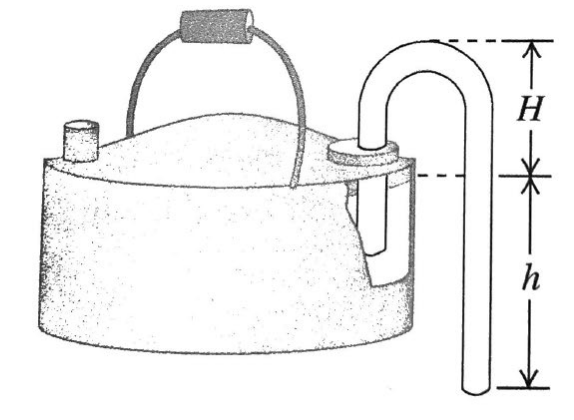
\includegraphics[width=0.5\linewidth]{../figures/P12_88.png}
  \label{fig:P12_88}
\end{figure}

A \textit{siphon} (\textbf{\autoref{fig:P12_88}}) is a convenient device for removing liquids from containers. To establish the flow, the tube must be initially filled with fluid. Let the fluid have density $\rho$, and let the atmospheric pressure be $p_{atm}$. Assume that the cross-sectional area of the tube is the same at all points along it.

\subsection*{(a)}
If the lower end of the siphon is at a distance $h$ below the surface of the liquid in the container, what is the speed of the fluid as it flows out the lower end of the siphon? Assume that the container has a very large diameter, and ignore any effects of viscosity)
\bigbreak
\begin{figure}[ht]
  \centering
  \incfig[0.6]{A7P3}
  \caption{Fritlegemediagram}
  \label{fig:A7P3}
\end{figure}
\bigbreak
Fra Bernoullis ligning har vi, idet vi sætter $h = 0$ ved $C$, at
\[ 
p_A + \frac{1}{2}\rho v_A^2 + \rho gh = p_C + \frac{1}{2}\rho v_C^2 + 0
.\]
Vi har generelt for væsker i bevægelse at $v \sim \frac{1}{A}$ og dermed har vi at for den store cylinder med stort overfladeareal $A_A$ en hastighed $v_A \approx 0$. Vi får dermed følgende simplificering
\[ 
p_A + \rho gh = p_C + \frac{1}{2}\rho v_C^2
.\]
Hastigheden ved punkt $C$ $v_C$ kan nu isoleres
\[ 
  v_C = \sqrt{2\frac{p_A + \rho gh - p_C}{\rho}}
.\]
Idet vi for tilfældet i opgaven har at $p_A = p_C$ fås
\[ 
v_C = \sqrt{2gh}
.\]
Altså er hastigheden af væsken i punkt $C$, \underline{\underline{$v_C = \sqrt{2gh}$}}. Dette stemmer overens med det generelle resultat at væsker falder med den almindelige fritfaldshastighed for en trykforskel $\Delta p = 0$.


\subsection*{(b)}
A curious feature of a siphon is that the fluid initially flows ``uphill''. What is the greatest height $H$ that the high point of the tube can have if flow is still to occur.
\bigbreak
Her kan Bernoullis ligning også opskrives, denne gang sættes $h = 0$ dog til højden på vandoverfladen (punkt $A$). Vi får altså
\[ 
p_B + \rho gH + \frac{1}{2}\rho v_B^2 = p_C + \rho g (-h) + \frac{1}{2} \rho v_C^2
.\]
Fra bevarelse af strømningshastigheden har vi at
\[ 
A_B v_B = A_C v_C
.\]
Idet $A_B = A_C$ må det også gælde at $v_B = v_C$. Altså reduceres Bernoullis ligning til
\[ 
p_B + \rho gH = p_C + \rho g(-h)
.\]
Desuden gælder at ethvert tryk aldrig kan blive mindre end \qty{0}{Pa}. Altså må det gælde at $p_B > 0$ for at \textit{siphonen} kan virke. Dermed fås at
\begin{align*}
  p_B &= p_C + \rho g(-h) - \rho g H \\
  0 &< p_C + \rho g (-h) - \rho g H \\
  \rho g H &< p_C + \rho g (-h) \\
  H &< \frac{p_C - \rho g (-h)}{\rho g} \\
  H &< \frac{p_C}{\rho g} - h
.\end{align*}
Idet vi indsætter $p_C = p_{atm}$ fås at \textit{siphonen} virker når \underline{\underline{$ H < \frac{p_{atm}}{\rho g} - h$}}.

\begin{figure}[ht]
    \centering
    \incfig{jesus}
    \caption{jesus}
    \label{fig:jesus}
\end{figure}

\end{document}
